
%(BEGIN_QUESTION)
% Copyright 2006, Tony R. Kuphaldt, released under the Creative Commons Attribution License (v 1.0)
% This means you may do almost anything with this work of mine, so long as you give me proper credit

A vessel contains three different liquids of different specific gravities: glycerine, water, and olive oil.  These three liquids settle at different levels in the vessel, so that there is a 3 foot deep layer of glycerine, a 2 foot deep layer of water, and a 4.5 foot deep layer of olive oil:

$$\includegraphics[width=15.5cm]{i00235x01.eps}$$

Calculate the total hydrostatic pressure at the bottom of the vessel, in units of PSI and kPa.

\underbar{file i00235}
%(END_QUESTION)





%(BEGIN_ANSWER)

Hydrostatic pressure due to 3 feet of glycerine (SG = 1.26)

\vskip 10pt

(1.26)(3 feet)(12 in / 1 ft)(1 PSI / 27.6807 "W.C.) = 1.639 PSI

\vskip 20pt

Hydrostatic pressure due to 2 feet of water (SG = 1.00)

\vskip 10pt

(1.00)(2 feet)(12 in / 1 ft)(1 PSI / 27.6807 "W.C.) = 0.867 PSI

\vskip 20pt

Hydrostatic pressure due to 4.5 feet of olive oil (SG = 0.918)

\vskip 10pt

(0.918)(4.5 feet)(12 in / 1 ft)(1 PSI / 27.6807 "W.C.) = 1.791 PSI

\vskip 20pt

Total hydrostatic pressure = 1.639 PSI + 0.867 PSI + 1.791 PSI = 4.297 PSI = 29.6 kPa

%(END_ANSWER)





%(BEGIN_NOTES)

See question {\tt i00232.tex} for a list of common fluids' specific gravities.

%INDEX% Physics, static fluids: hydrostatic pressure

%(END_NOTES)


